\chapter{Projekt systemu}
\thispagestyle{chapterBeginStyle}

{\color{dgray}
W tym rozdziale przedstawiono szczegółowy projekt systemy w notacji UML uwzględniający wymagania funkcjonalne opisane w rozdziale~\ref{rozdzial1}. Do opisu relacji pomiędzy składowymi systemu wykorzystano diagramy \ldots.
Przedstawiono w pseudokodzie i omówiono algorytmy generowania \ldots.
}


\section{Grupy użytkowników i założenia}

{\color{dgray}
Architektura systemu \ldots jest wielowarstwowa i rozproszona, przy czym \ldots. Podsystem  \ldots jest systemem zbiorczym dla danych \ldots wysyłanych do serwera \ldots. 

Taka architektura jest zgodna z wzorcem projektowym MVC\footnote{Należy odnieść się do wykorzystywanych wzorców projektowych} (ang.  Model-View-Controller). Przetwarzanie danych odbywa się \ldots.
} 

\section{Przypadki użycia i scenariusze}
Jak zostało zdefiniowane w poprzednim punkcie, w pracy przewidziano 3 grupy użytkowników. W zamyśle framework jest narzędziem dla programisty, jednak w systemie został zaimplementowany szereg rozwiązań gotowych do wykorzystania dla końcowych użytkowników, dlatego diagramy przypadków użycia zostały podzielone na trzy klasy: 
\begin{itemize}
	\item przypadki użycia Programisty 
	\item przypadki użycia Użytkownika Administracyjnego potencjalnego serwisu e-commerce, opartego na opisywanym Frameworku
	\item przypadki użycia użytkownika końcowego, czyli Klienta
\end{itemize}

Na rysunku \ref{useCaseProgrammer} zostały przedstawione najważniejsze przypadki użycia frameworku. Programista ma swobodny dostęp do rozszerzania encji, w szczególności klasy Produkt, która ma wyjatkowo strategiczne znaczenie w systemach e-commerce. 

\begin{figure}[h!]
	\begin{center}
		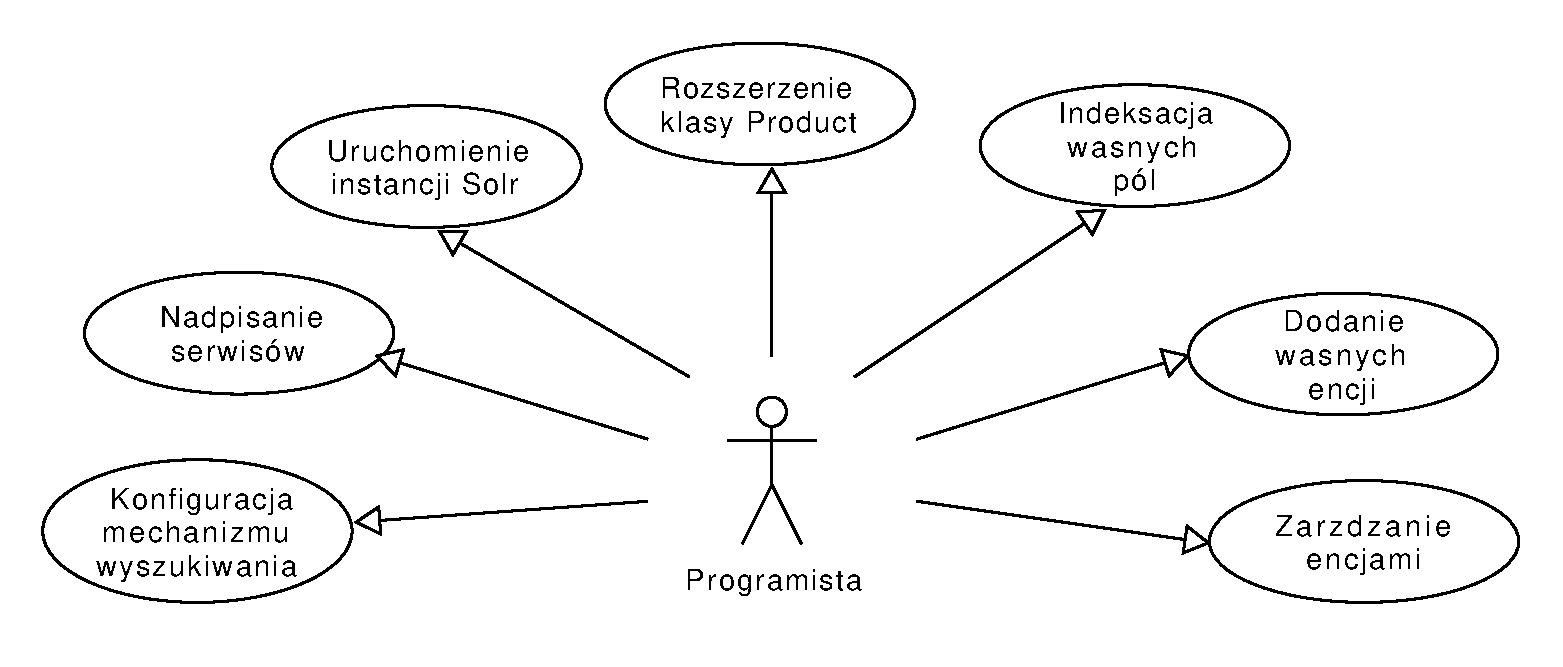
\includegraphics[width=1\textwidth]{ucdev.pdf}
	\end{center}
	\caption{{\color{black}Diagram przypadków użycia związany z Programistą.}} \label{useCaseProgrammer}
\end{figure} 

\begin{figure}[h!]
	\begin{center}
		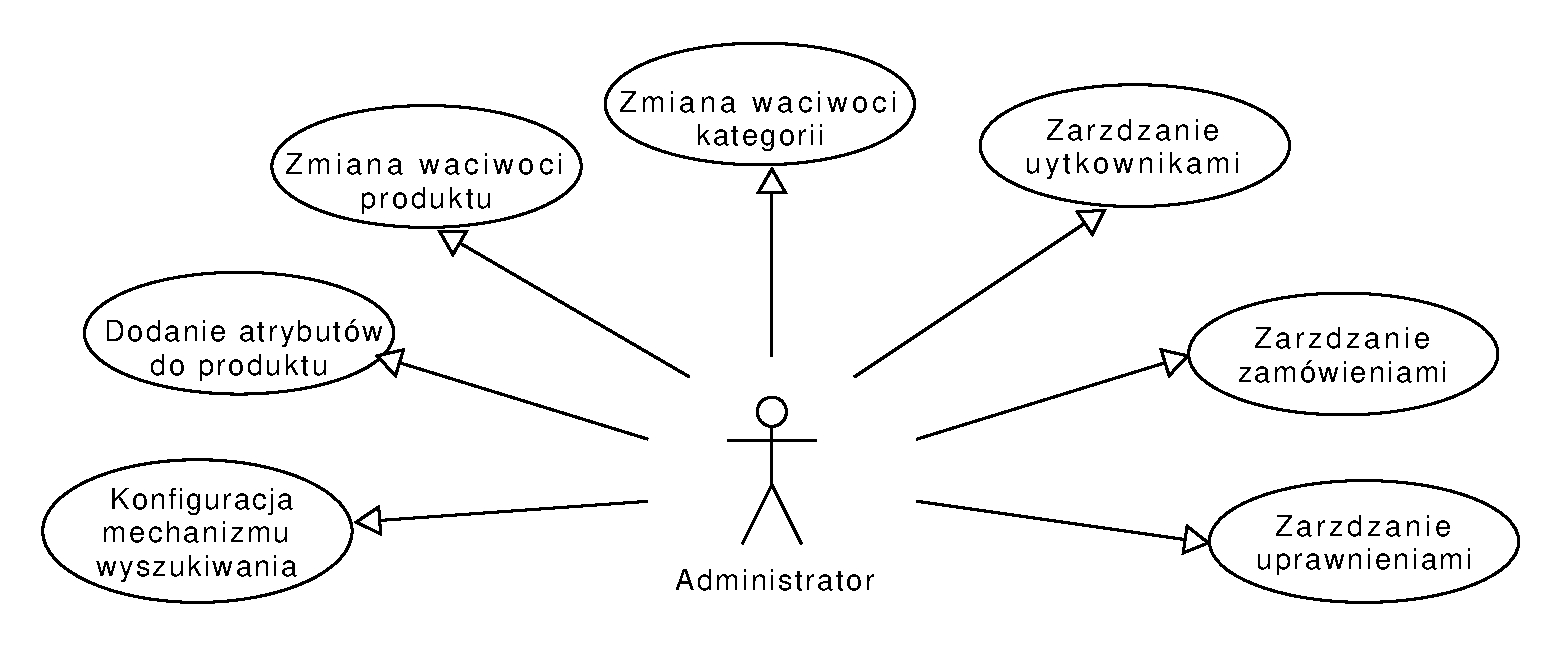
\includegraphics[width=1\textwidth]{ucadmin.pdf}
	\end{center}
	\caption{{\color{black}Diagram przypadków użycia związany z Administratorem ewentualniego systemu.}} \label{useCaseProgrammer}
\end{figure} 

\section{Diagramy klas}

W tej sekcji należy przedstawić diagramy klas dla odpowiednich elementów systemu zidentyfikowane na podstawie wcześniejszych rozważań 

\section{Diagramy aktywności}

W tej sekcji należy przedstawić diagramy aktywności dla elementów systemu i odpowiednich procesów wynikające z wcześniejszej analizy.  

{\color{dgray}
W niniejszym rozdziale przedstawiono diagramy aktywności \ldots. Diagram na rysunku~\ref{czynnosci_GD} przedstawia \ldots.
} 

\begin{figure}[h!]
\begin{center}
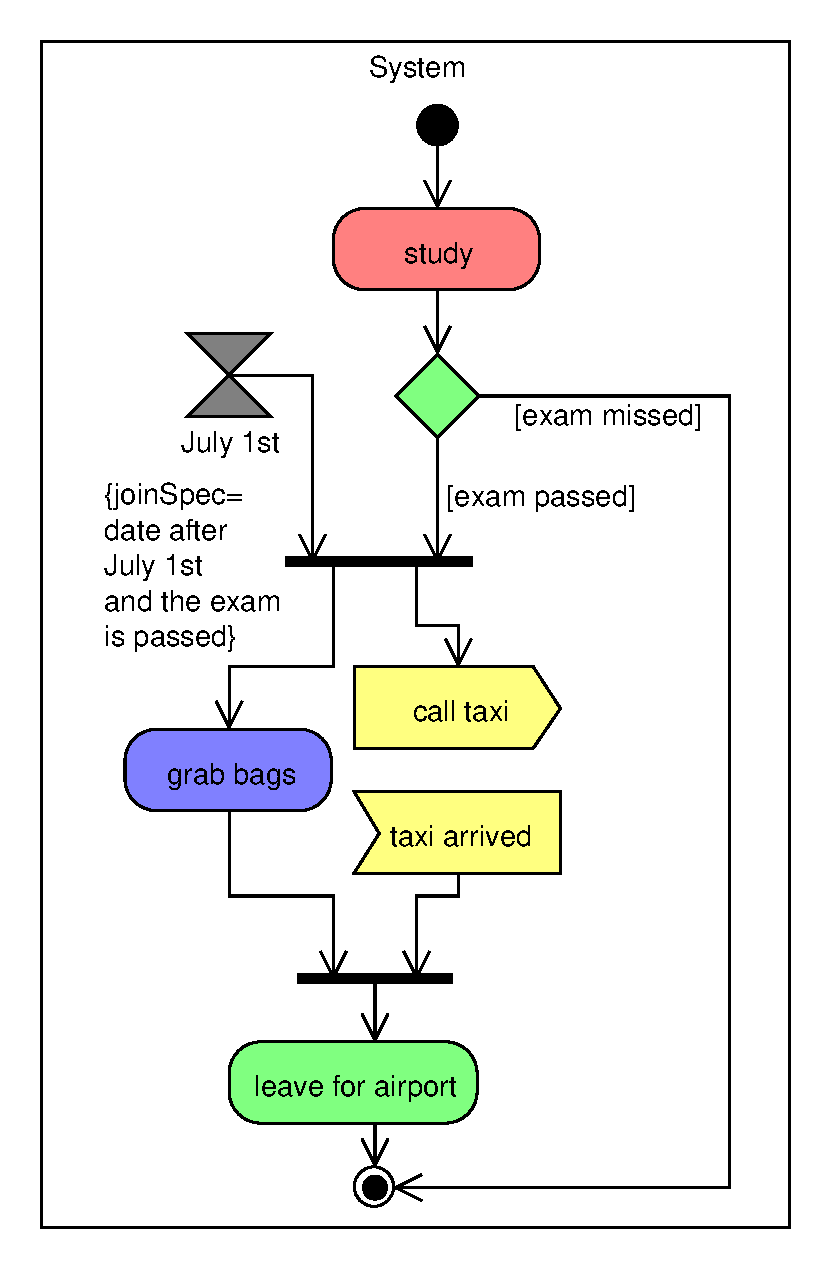
\includegraphics[width=0.5\textwidth]{aktyw.pdf}
\end{center}
\caption{{\color{dgray}Diagram aktywności związany z procesem rejestracji dokumentu.}} \label{czynnosci_GD}
\end{figure}  

\section{Diagramy sekwencji}

W tej sekcji należy przedstawić diagramy sekwencji dla obiektów systemu zidentyfikowanych na podstawie wcześniejszych rozważań. Należy wykorzystać nazewnictwo wprowadzone w poprzednich rozdziałach, w szczególności odpowiadające definicjom wprowadzonych klas.

\section{Diagramy stanów}

W tej sekcji należy przedstawić diagramy stanów w których może znaleźć się system. Diagramy te są szczególnie istotne przy projektowaniu systemów czasu rzeczywistego. 

\section{Projekt bazy danych}

W tej sekcji należy przedstawić projekt bazy danych. Należy omówić wycinek rzeczywistości i odpowiadające mu zidentyfikowane elementy systemu, których wartości będą podlegać utrwalaniu. Należy przedyskutować wybór typów danych dla atrybutów poszczególnych obiektów. Należy uzasadnić wybór platformy DBMS. Dla relacyjnych baz danych należy przedyskutować jej normalizację.

\section{Opis protokołów}

W tej sekcji należy omówić protokoły wykorzystywane przez komponenty systemu. Omówić formaty komunikatów i zilustrować je przykładami. 

\section{Opis algorytmów}

W tej sekcji należy wymienić i przedyskutować algorytmy wykorzystywane w systemie. Algorytmy należy przedstawić w pseudokodzie (wykorzystać pakiet \texttt{algorithm2e}). Omówienia poszczególnych kroków algorytmów powinny zawierać odwołania do odpowiednich linii pseudokodu. Dla zaproponowanych autorskich algorytmów należy przeprowadzić analizę ich złożoności czasowej i pamięciowej. 

{\color{dgray}
Algorytm bąblowania jest przedstawiony w Pseudokodzie~\ref{alg:mine}.
}

{\small
\begin{pseudokod}[H]
%\SetAlTitleFnt{small}
\SetArgSty{normalfont}
\SetKwFunction{Process}{Process}
\SetKwFunction{Calculate}{Calculate}
\KwIn{Zbiór bąbli $B$}
\KwOut{Wyporność $W$}
\ForEach{$b \in B$}{
\Process{$b$}\;
\For{$i \leftarrow 1$ \KwTo $|B|$}{
\If{\Calculate{EW($i$,$b$)} $\le$ 0}{
$b \leftarrow 2*b$\;
}
}
}
\While{$B \neq \emptyset$}{
\For{$j \leftarrow 1$ \KwTo $|B|$}{
\If{\Calculate{FT($j$,$\hat{b}$)} $\le 0$}{
$w \leftarrow 2*\hat{b}$\;
$W \leftarrow W \cup \{w\}$\;
$B \leftarrow B \setminus \{b\}$\;
}
}
}
\caption{Wyporność przez bąblowanie}\label{alg:mine}
\end{pseudokod}
}

